% 2007 年浙江卷理科第 4 题：边长 16 米的正方形草坪与喷水龙头示意。
% 来源 PDF：gaokaomath-src/普通高考/2007/2007浙江理.pdf
% SHA-256：31c1d0d79ba11a3644a27b5ee3781f52caaf831209e8da63ddd8d7019cd06995
% 原页：2007浙江理.pdf 第 1 页（A3 三栏）第 1 栏，书页码 417。
% 重绘依据：按原页正方形草坪与中心喷水圆面的透视重绘。
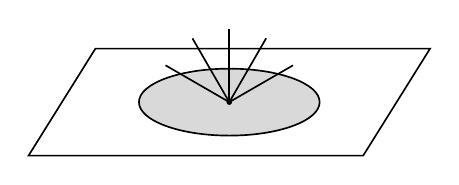
\begin{tikzpicture}[scale=0.85, semithick,
  every node/.style={inner sep=1pt}]

  % 正方形草坪（斜投影）
  \draw (0,0) -- (5,0) -- (6,1.6) -- (1,1.6) -- cycle;

  % 喷水圆面
  \fill[gray!30] (3,0.8) ellipse (1.35 and 0.5);
  \draw (3,0.8) ellipse (1.35 and 0.5);
  \fill (3,0.8) circle (1.2pt);

  % 水花射线
  \foreach \a in {30,60,90,120,150} {
    \draw (3,0.8) -- ++(\a:1.1);
  }
\end{tikzpicture}
